\documentclass{article}
\usepackage{setspace}
\usepackage{graphicx}
\usepackage{subfigure}
\usepackage{amsmath}
\usepackage{pythonhighlight}
\usepackage{longtable}
\usepackage{booktabs}
\usepackage{geometry}
\usepackage{xcolor}
\usepackage{caption}
\usepackage{amsfonts,amssymb}
\usepackage{multirow}
\usepackage{subfigure}
\geometry{a4paper,scale=0.8}
\begin{document}
\begin{titlepage}
	\begin{center}
		\vspace*{1cm}
		\Large{\textbf{DSA5103}}\\
		\Large{\textbf{Optimization algorithms for data modelling}}\\
		\vspace{1cm}
		\small
		National University of Singapore\\
		Data Science and Machine Learning Department\\
		\today \\
		\vfill
		%School of Mathematics and Science\\
		%Soochow University \\
		%\line(1,0){400}\\[1mm]
		\LARGE{\textbf{Assignment 2}}\\[5mm]
		%\Large{\textbf{-The Research on Students' Admission-}}\\[1mm]
		%\line(1,0){400}
		\vfill
		\small
		Wang Jiangyi, A0236307J\\
		e0732857@u.nus.edu
	\end{center}
\end{titlepage}
\section{Question 1, Slater + KKT}
\begin{equation}
	\label{eq1}
	\begin{split}
		min_x:-\sum_{i=1}^{n} log(1+x_i)
		\\ s.t:\ x_i \ge 0, \quad i\in [n] \quad
		\\ \sum_{i=1}^n x_i = 1 \quad \quad \quad
	\end{split}
\end{equation}
\subsection{Slater's condition}
Firstly, recap that, Slater's condition is, find $\hat{x}\in \mathbb{R}^n $ such that,
\begin{equation}
	\nonumber
	\begin{cases}
		\  \sum_{i=1}^n \hat{x}_i = 1 \\
		\  \hat{x}_i > 0,\ i\in [n]
	\end{cases}
\end{equation}
This exactly holds since we can choose $\hat{x}=[\frac{1}{n},...,\frac{1}{n}]^T\in \mathbb{R}^n$, then we can check,
\begin{equation}
	\nonumber
	\begin{cases}
		\  \sum_{i=1}^n \frac{1}{n}  =n\times \frac{1}{n} = 1 \\
		\  \hat{x}_i=\frac{1}{n} > 0,\ i\in [n]
	\end{cases}
\end{equation}
Therefore, Slater's condition holds. 
\vspace{4pt}
\\
\underline{[This part is not required for this problem]} Moreover, Optimization problem (\ref{eq1}) is indeed one \textbf{Convex Programming}. Based on that, i.e., \textbf{convex programming and slater's condition}, it implies that \textbf{Strong Duality holds} for Optimization problem (\ref{eq1}). Suppose that we make the following notation,
\begin{equation}
	\nonumber
	\begin{cases}
	 \ 	f(x) =-\sum_{i=1}^{n} log(1+x_i) \\
	 \ 	g(x) = \mathbb{I}^Tx-1 \\
	\  	h_i(x) = -x_i, \ i \in [n]
	 \end{cases}
\end{equation} 
After simple calculation, we have,
\begin{equation}
	\nonumber
	\nabla^2 f(x) = Diag\left\{ \frac{1}{(1+x_1)^2},...,\frac{1}{(1+x_n)^2}\right\}\succ 0
\end{equation}
Therefore, we have, $f(\cdot)$ is convex; $g(\cdot)$ is affine; $h_i(\cdot)$ is affine (thus convex). This shows Optimization problem (\ref{eq1}) is exactly a \textbf{convex programming}, implying that \textbf{Strong Duality holds}.
\subsection{KKT condition}
Denote Lagrangian function as $L(x;u,v)$, then we have:
\begin{equation}
	\nonumber
	L(x;u,v) = -\sum_{i=1}^n log(1+x_i) -\sum_{i=1}^{n} u_i x_i + v(1-\sum_{i=1}^{n}x_i)
\end{equation}
Therefore, KKT condition $($at $x=x^*)$ with respect to dual variable $(u=u^*, v=v^*)$ is,
\vspace{4pt}
\\
1. Stationarity Condition:
\begin{equation}
	\nonumber
	\nabla_{x_i}L(x^*;u^*,v^*) = 0 \implies -\dfrac{1}{1+x_i^{*}} -u_i^* - v^* =0, \ i\in [n]
\end{equation}
\\
2. Primal Feasibility Condition:
\begin{equation}
	\nonumber
	\begin{cases}
		\ \sum_{i=1}^{n}x_i^*=1 \\
		\ x_i^* \ge 0,\ i\in[n]
	\end{cases}
\\
\end{equation}
\\
3. Dual Feasibility Condition:
\begin{equation}
	\nonumber
	\begin{cases}
			\ u_i^* \ge 0,\ i\in[n] \\
		\ v^* \in \mathbb{R}
	\end{cases}
\end{equation}
\\
4. Complementary Slackness Condition:
\begin{equation}
	\nonumber
	u_i^*x_i^*=0,\ i\in [n]
\end{equation}
All \underline{(1-4) conditions} (Stationarity, Primal Feasibility, Dual Feasibility, Complementary Slackness) contribute to the whole KKT condition.
\vspace{4pt}
\\
\underline{[This part is not required for this problem]} In Section 1.1, we show that, \textbf{Strong Duality holds }and \textbf{Optimization problem (\ref{eq1}) is Convex Programming}. Therefore, it is sufficient to show, $(x^*;u^*,v^*)$ is the optimal solution to $(Primal\  problem;Dual \ problem)$ if and only if, KKT condition is satisfied $($at $x=x^*)$ with respect to dual variable $(u=u^*, v=v^*)$.
\vspace{4pt}
\\
This result builds the connection between 'dual optimal solution' and 'primal optimal solution' with the help of 'KKT condition'.
\section{Question 2, Coordinate Descent}
\begin{equation}
	min_x: f(x_1,x_2) = 2x_1^2 - 6x_1x_2 + 5x_2^2-4x_1-3x_2
\end{equation}
To better apply Coordinate Descent Algorithm, let us find general exact solutions for the following coordinate-wise optimization problem:
\begin{equation}
	\nonumber
	\begin{cases}
	\ 	\hat{x}_2 = argmin_{x_2} :f(a,x_2) = argmin_{x_2}: 5x_2^2 -(3+6a)x_2 \\
	\ 	\hat{x}_1 = argmin_{x_1}: f(x_1, b) = argmin_{x_1}: 2x_1^2 - (4+6b) x_1
	\end{cases}
\end{equation}
Based on \underline{Convexity of $f(\cdot)$ and Second-order Optimality Condition}, we can easily achieve the following update formular of $(\hat{x}_1, \hat{x}_2)$,
\begin{equation}
	\nonumber
	\begin{cases}
		\ 	\hat{x}_2 = \frac{1}{10}\cdot(3+6x_1) \\
		\ 	\hat{x}_1 = \frac{1}{2}\cdot(2+3x_2)
	\end{cases}
\end{equation}
Therefore, starting from $x^{(0)} =\begin{bmatrix}
	0
	\vspace{1pt}
	\\
	0
 \end{bmatrix}$we have:
\begin{equation}
	\nonumber
	\begin{cases}
		\ 	x_1^{(1)} = \frac{1}{2}\cdot(2+3x_2^{(0)}) =  \frac{1}{2} \cdot 2 =1 \\
		\ 	x_2^{(1)} = \frac{1}{10}\cdot(3+6x_1^{(1)} = \frac{1}{10} \cdot 9 = \frac{9}{10})
	\end{cases}
\end{equation}
\begin{equation}
	\nonumber
	\begin{cases}
		\ 	x_1^{(2)} = \frac{1}{2}\cdot(2+3x_2^{(1)}) =  \frac{1}{2} \cdot \frac{47}{10} =\frac{47}{20} \\
		\ 	x_2^{(2)} = \frac{1}{10}\cdot(3+6x_1^{(2)} = \frac{1}{10} \cdot \frac{171}{10} = \frac{171}{100})
	\end{cases}
\end{equation}
To conclude, we attain: $x^{(1)} =\begin{bmatrix}
	1
	\vspace{3pt}
	\\
	\dfrac{9}{10}
\end{bmatrix}$, $x^{(2)} = \begin{bmatrix}
\dfrac{47}{20}
\vspace{6pt}
\\
\dfrac{171}{100}
\end{bmatrix}$
\section{Question 3, LASSO}
\begin{equation}
	min_{\beta} : \frac{1}{2}||X\beta - Y|| + \lambda||\beta||_1
\end{equation}
Here, $X\in \mathbb{R}^{n\times p}$, $\beta \in \mathbb{R}^p$ and $n=1000$, $p=5000$. The ground truth label $Y$ is generated by,
\begin{equation}
	\nonumber
	Y = X\beta^* + 0.01\epsilon
\end{equation}
$\beta^*$ is a sparse vector, with only 5\% non-zero entries. $X_{ij} \sim N(0,1)$ and $\epsilon \sim N(\mathbf{0}_n,\mathbb{I}_n)$.
\newpage
\subsection{Relative Residual Error v.s. Iteration Number}
The result can be shown as follows:
\begin{figure}[h]
	\centering
	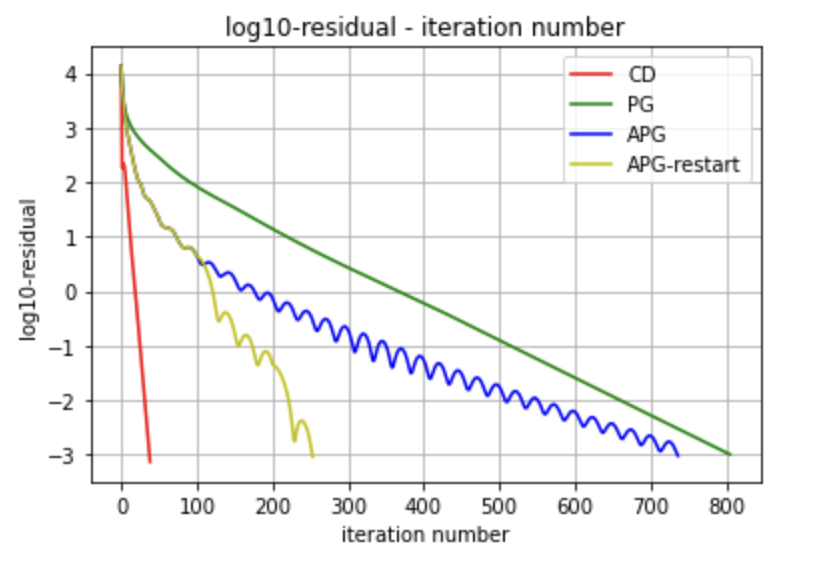
\includegraphics[width=.35\textheight]{c.png}
	\caption{Relative Residual Error v.s. Iteration Number}
	\label{fig:001}
\end{figure}
\\
\textbf{Explanation}:
\vspace{4pt}
\\
1. CD method achieves '1e-3' relative residual error with the smallest iteration number. Possible reason is, CD  method solves \textbf{exact} coordinate-wise minimization problem. From this perspective, CD method will not twist orginal objective too much. This also leads to the\textbf{ strict decrease} for residual error.
\\
2. As for PG method, the residual error also \textbf{decreases strictly}. That is because, PG method can be viewed as one variation of GD method. Suppose that the step length is small enough, then we can guarantee the strict decrease in GD framework. For APG and APG-restart method, \textbf{this never happen}s due to the momentum term. However, the momentum term can accelerates the algorithm convergence rate.
\\
3. Compared with APG, APG-restart converges faster since the restart mechanism. As the training goes on, $t_k \rightarrow \infty$ and we utilzie too many $\Delta \beta$ information, which will slow down the convergence. This is why we need to restart the $t_k$ to accelerate the convergence.
\\
4. In the beginning stage of APG and APG-restart, it is almost the same with PG since the weight for $\Delta \beta$ term is extremely small.
\subsection{Relative Residual Error v.s. Running Time}
The result is shown as follows:
	\begin{figure}[h]
	\centering
	\subfigure[without CD method]{
		\label{fig:subfig:a} %% label for first subfigure
		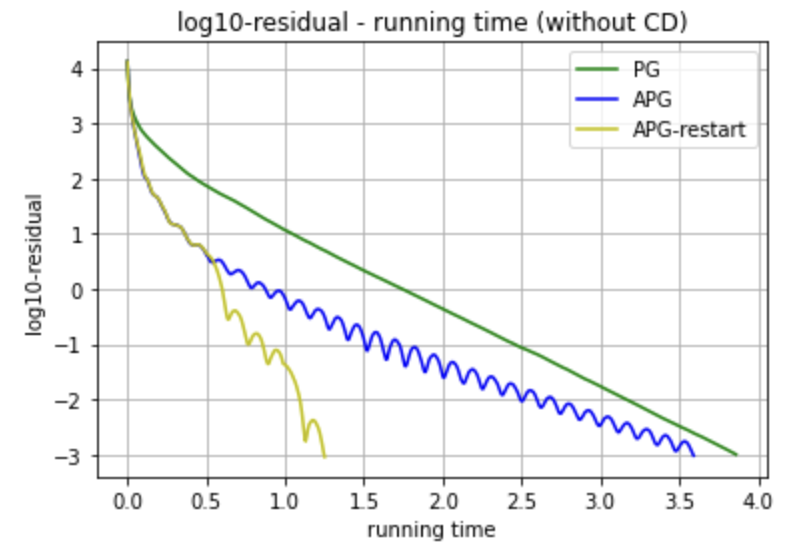
\includegraphics[width=2.8in]{d1.png}}
	\subfigure[with CD method]{
		\label{fig:subfig:b} %% label for second subfigure
		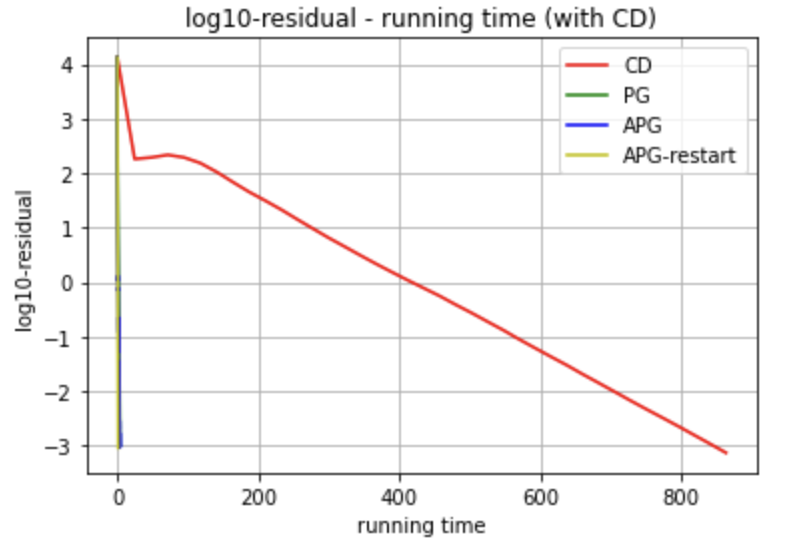
\includegraphics[width=2.8in]{d2.png}}
	\caption{Relative Residual Error v.s. Running Time}
	\label{fig:002} %% label for entire figure
\end{figure}
\\
\textbf{Observation}:
\vspace{4pt}
\\
1. For PG, APG and APG-restart algorithm, the running time is approximately propotional to the iteration number. Moreover, compared with CD method, these 3 algorithms are extremely fast, at the cost of more iteration number.
\\
2. For CD method, it is extremely slow. Reason is, although it requires small number of iteration to achieve '1e-3' residual error, within each iteration, it requires to update each entry of $\beta$ sequentially (cannot parallelize).
\subsection{APG, APG-restart Examination}
The report of relative residual error, iteration and time of APG, APG-restart is shown as follows,
\begin{figure}[h]
	\centering
	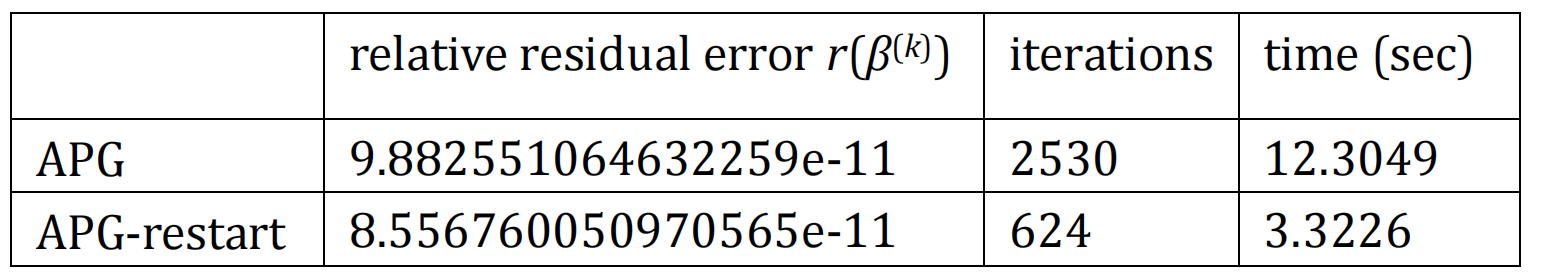
\includegraphics[width=.35\textheight]{e.png}
	\caption{Relative Residual Error, Iteration, Time for APG, APG-restart}
	\label{fig:003}
\end{figure}
\\
To conclude, for both APG and APG-restart, we are able to achieve '1e-10' relative residual error within 3000 iteration. However, APG-restart is faster than APG.
\subsection{Choices of step length $\alpha$}
The result is, for both $\alpha = \frac{1}{L}$ and $\alpha = \frac{1.5}{L}$, APG and APG-restart will converge. Moreover, for $\alpha = \frac{1.5}{L}$, algorithms (both APG and APG-restart) will converge faster! The diagram can be shown as follows,
\begin{figure}[h]
	\centering
	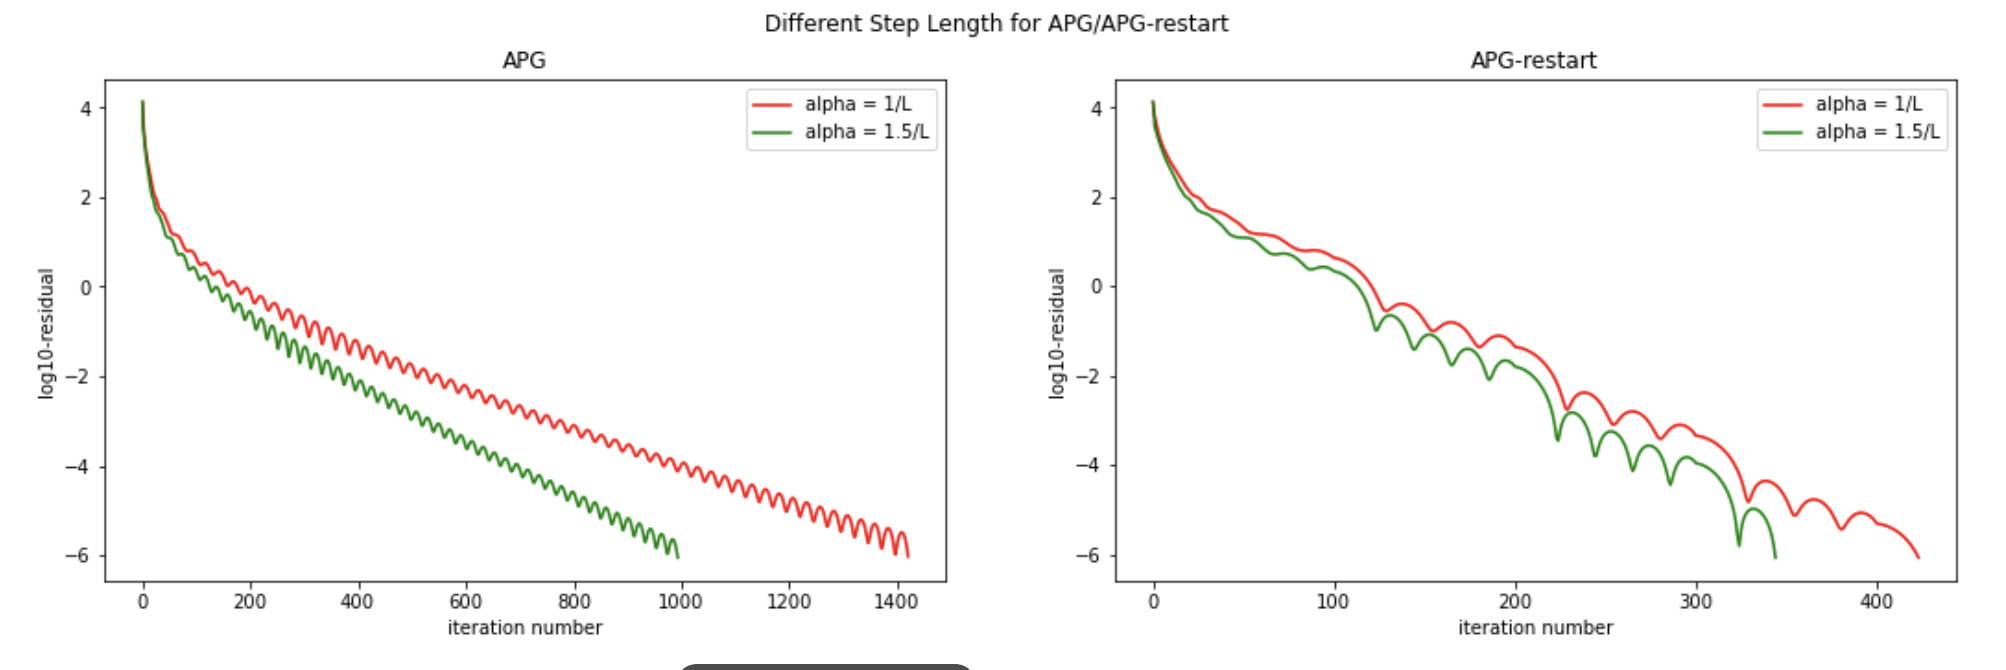
\includegraphics[width=.55\textheight]{f1.png}
	\caption{Different Step Length $\alpha$ for APG/APG-restart}
	\label{fig:004}
\end{figure}
\\
From Figure \ref{fig:004}, it can be observed that, after increasing $\alpha$ from $\frac{1}{L}$ to $\frac{1.5}{L}$ (1.5 times), we only require $\frac{1}{1.5} = \frac{2}{3}$ times iteration.
\vspace{4pt}
\\
However, this does not mean we can arbitrarily enlarge the $\alpha$, which will make the algorithm diverge. Here, we make one experiment, setting $\alpha = \frac{3}{L}$. Then the residual error starts to diverge, which can be shown as follow,
\begin{figure}[h]
	\centering
	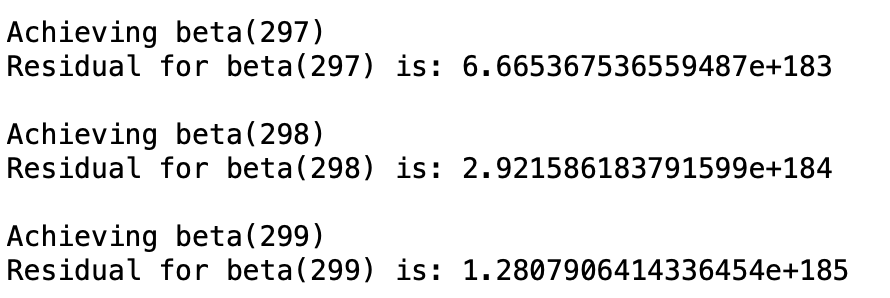
\includegraphics[width=.4\textheight]{f2.png}
	\caption{$\alpha = \frac{3}{L}$ for APG-restart Method}
	\label{fig:005}
\end{figure}
\\
This illustrates that, when setting $\alpha = \frac{3}{L}$, after 300 iteration, the Relative Residual Error grows to 1e185. \textbf{That is to say, the algorithm will diverge when step length is large enough.}
\end{document}